
\subsection{Flatt\'e function for the $\Xone$ and $Z_{cs}(4000)$ components}
\label{sec:flatte}

As demonstrated in Appendix \ref{SUPPsec:threshold}, 
only $X(4140)$ and $Z_{cs}(4000)$ peak not far from the coupled-channel thresholds of right $J^P$ values in S-wave (higher angular momenta are suppressed for threshold effects). 
In this section,
possible impact of these thresholds is investigated.

Since $\Xone$ peaks near the $\jpsi\phi$ kinematic threshold, 
decays to lighter particle combinations can have a significant impact on its line shape.
As a $1^+$ state $\Xone$ should easily decay via $S-$wave to $D_s^{*\pm}D_s^{\mp}$ which has the lower mass threshold than $\jpsi\phi$.
As an alternative to our nominal fit, 
in which mass dependence of $\Xone$ width is neglected, 
in this section,
mass-dependent width with both channels included is explored. 
The Breit-Wigner formula $BW(m)$ is replaced by the Flatt\'e model: 
\begin{equation}
{\rm Flatte}_X(m|M_0\,,g_{\jpsi\phi}\,,g_{D_s^*D_s})=\frac{1}{M_0^2-m^2-iM_0(g_{\jpsi\phi}\rho_{\jpsi \phi}+g_{D_s^*D_s}\rho_{D_s^*D_s})},
\label{eq:fl}
\end{equation}
where the parameters $g_i$ are the $\Xone$ coupling constants to channel $i$, 
the phase-space factors $\rho_i=2p_i/m$ are dependent on $m\equiv\mjf$ and on momentum $p_i$ of one of the daughters in channel $i$. 
The $\mjf$ mass projections of the fits with $\Xone$ in the Flatt\'e parameterizations for different models of the other components are shown in Fig.~\ref{fig:flatte}. 
The fit parameters are given in Table~\ref{tab:flatte}.  
In term of fit likelihood, 
Flatt\'e parameterization is better than the constant-width Breit-Wigner function by about $\Delta(2\ln\Like)\sim20$ when the same resonance model is used. 
Since in the Flatt\'e model $p_i$ becomes imaginary below the kinematic threshold, 
the real part of the amplitude pole position is not necessarily equal to $M_0$. 
The pole position $m_{\rm pole}\equiv M_{\rm pole}- i\Gamma_{\rm pole}/2$ is obtained by solving the equation that the denominator in Eq.~(\ref{eq:fl}) becomes equal to zero when $m=m_{\rm pole}$. 
The results are also reported in Table~\ref{tab:flatte}. 
The pole of Flatt\'e fit corresponds to the 4th Riemann sheet. 
The $Z_{cs}(4220)$ with $J^P=1^{-}$ and $1^+$ hypotheses give similar fit likelihood and 2D $\chisq$ on Dalitz-plot $m^2_{\jpsi\phi}$ and $m^2_{\jpsi K}$ plane, 
and the fit results with $Z_{cs}(4220)$ in the $1^-$ hypothesis are also shown.
In all Flatt\'e fits, 
the coupling of $X(4140)$ to the coupled-channel is smaller than to the $\jpsi\phi$ and is insignificant. 


\begin{table}[hbtp]
\centering
\caption{Comparison for $\Xone$ resonance with Flatt\'e and constant-width Breit-Wigner functions. 
The numbers between horizontal bands, the first (second), correspond to $Z(4220)$ with $J^P=1^{-(+)}$.  
Also shown are the $\ln\Like$  and 2D $\chisq$ of Dalitz-plot distribution in the $m^2_{\jpsi\phi}$ vs.\ $m^2_{\jpsi K}$ plane with 1018 adaptive bins.}\label{tab:flatte}
\small{
\begin{tabular}{lccccccc}\hline
Flatt\'e&  $M_0$ (MeV)& $g_{\jpsi\phi}$ (GeV)& $g_{D_s^*D_s}/g_{\jpsi\phi}$ & Pole (MeV)&FF (\%)& $\ln\Like$& 2D $\chisq$\\\hline
Nominal & $  4202 \pm    18 $ & $  1.44 \pm  0.36 $ & $  0.05_{-0.05}^{+0.40} $  & $4092 - 90 i$ & $  19.1 $ &  5012.0 & 1022\\
Nominal & $  4223 \pm    29 $ & $  1.61 \pm  0.48 $ & $  0.06_{-0.06}^{+0.40} $ & $4082 - 113 i$ & $  17.7 $ &  5013.1 & 1039\\ 
\hline
Extended & $  4216 \pm   23 $ & $  1.46 \pm  0.44 $ & $  0.10_{-0.10}^{+0.40} $ & $4089 - 108 i$& $  35.3 $ &  5080.1 & 1001\\ 
Extended & $  4187 \pm   22 $ & $  1.06 \pm  0.49 $ & $  0.34_{-0.28}^{+0.40} $ & $4084 - 83 i$& $  21.0 $ &  5074.4 & 1027\\ 

\hline\hline
BW&  $M_0$ (MeV)& \multicolumn{2}{c}{$\Gamma$ (GeV)}& Pole (MeV) &FF (\%)& $\ln\Like$  & 2D $\chisq$\\\hline
Nominal & $  4116\pm 10 $ & \multicolumn{2}{c}{$   130 \pm 21 $} & $  4116 -    65 i $ & $  18.0 $ &  5001.6 & 1028\\ 
Nominal & $  4118\pm 14 $ & \multicolumn{2}{c}{$   162 \pm 22 $} & $  4118 -    81 i $ & $  17.4 $ &  5004.6 & 1044 \\ \hline
Extended & $  4107\pm 12 $ & \multicolumn{2}{c}{$   168 \pm 21 $} & $  4107 -    84 i $ & $  43.2 $ &  5070.4  & 1004\\ 
Extended & $  4108\pm 12 $ & \multicolumn{2}{c}{$   137 \pm 22 $} & $  4108 -    69 i $ & $  21.0 $ &  5068.7 & 1029\\ 
 
\hline
\end{tabular}
}
\end{table}

\begin{figure*}[t]
\centering
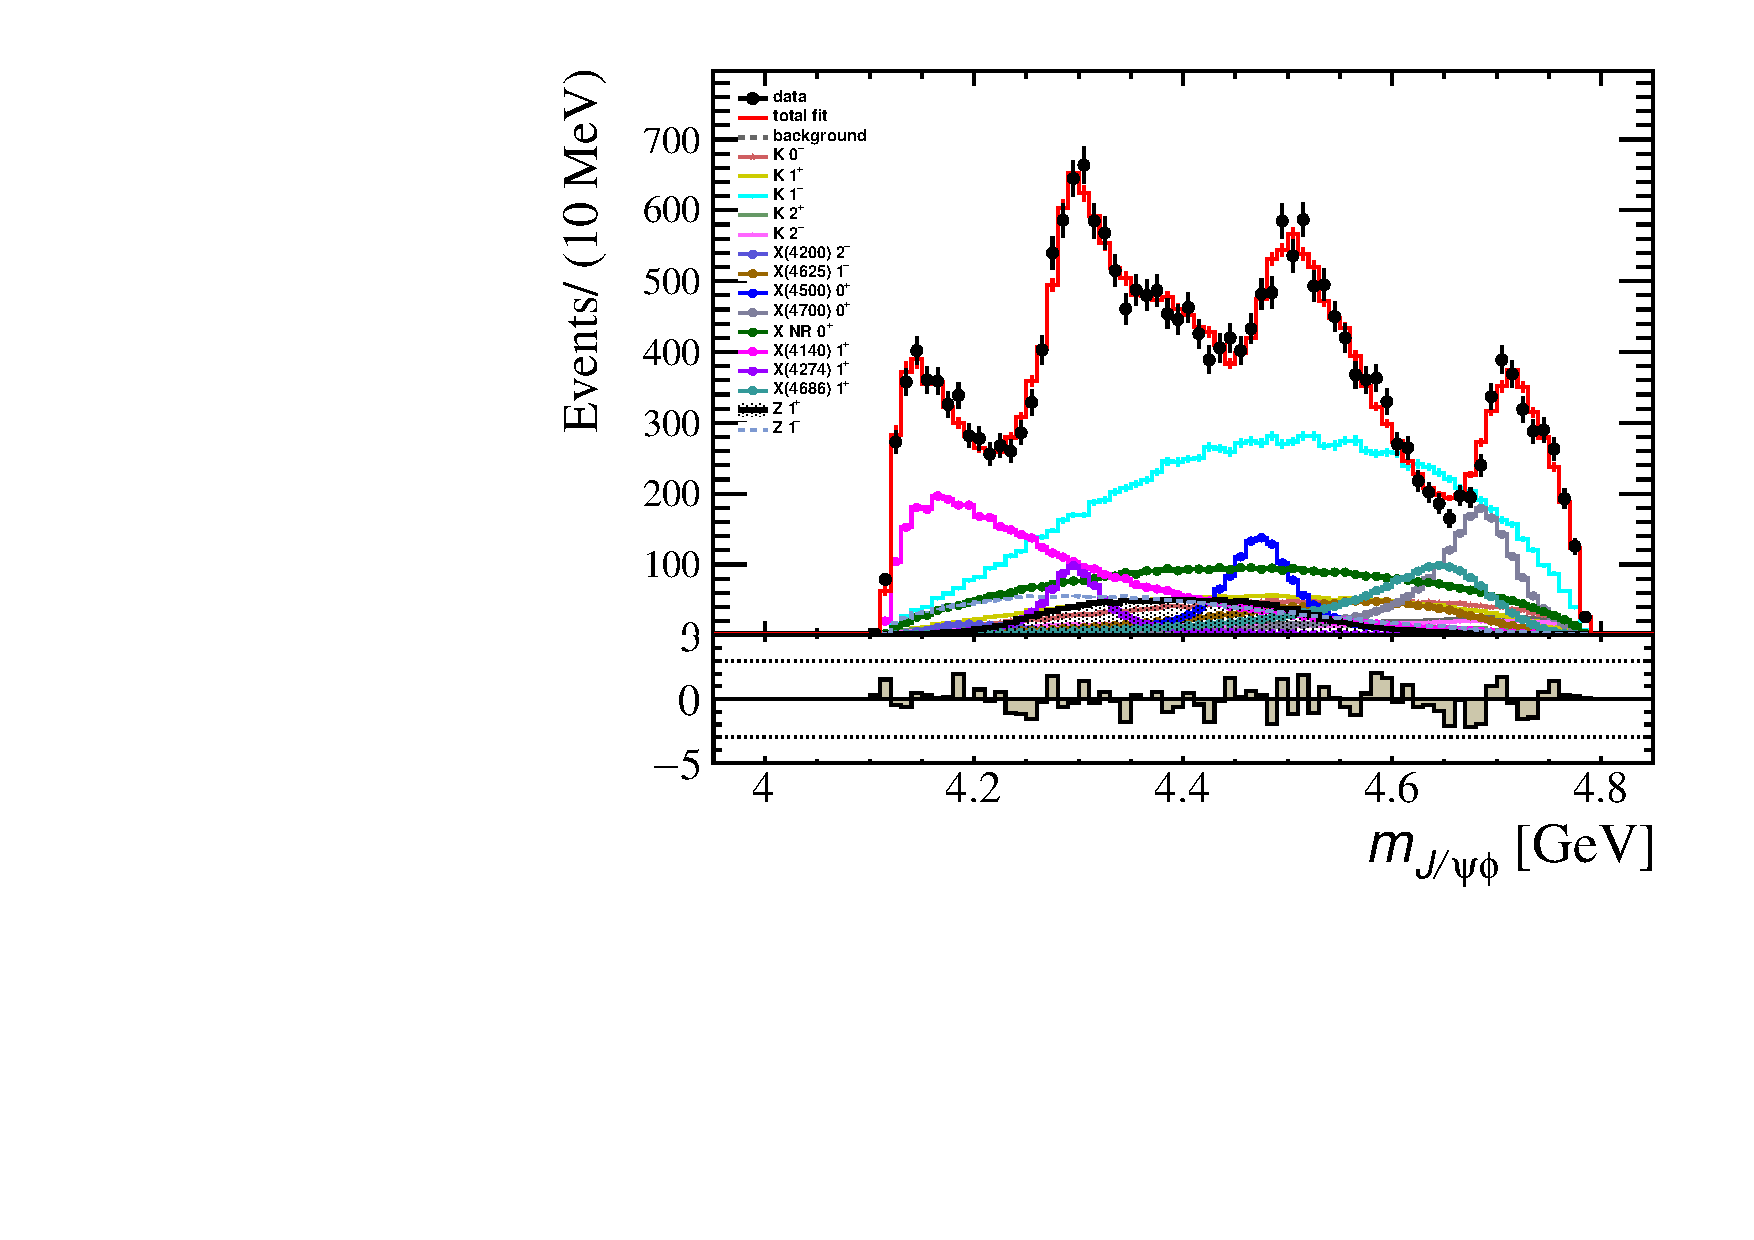
\includegraphics[width=0.5\textwidth]{Figures/06_Amplitude/Flatte/mjpsiphi-4140FL-Z1M}%
\put(-50,140) {\textrm{\small \bf(a)}}%
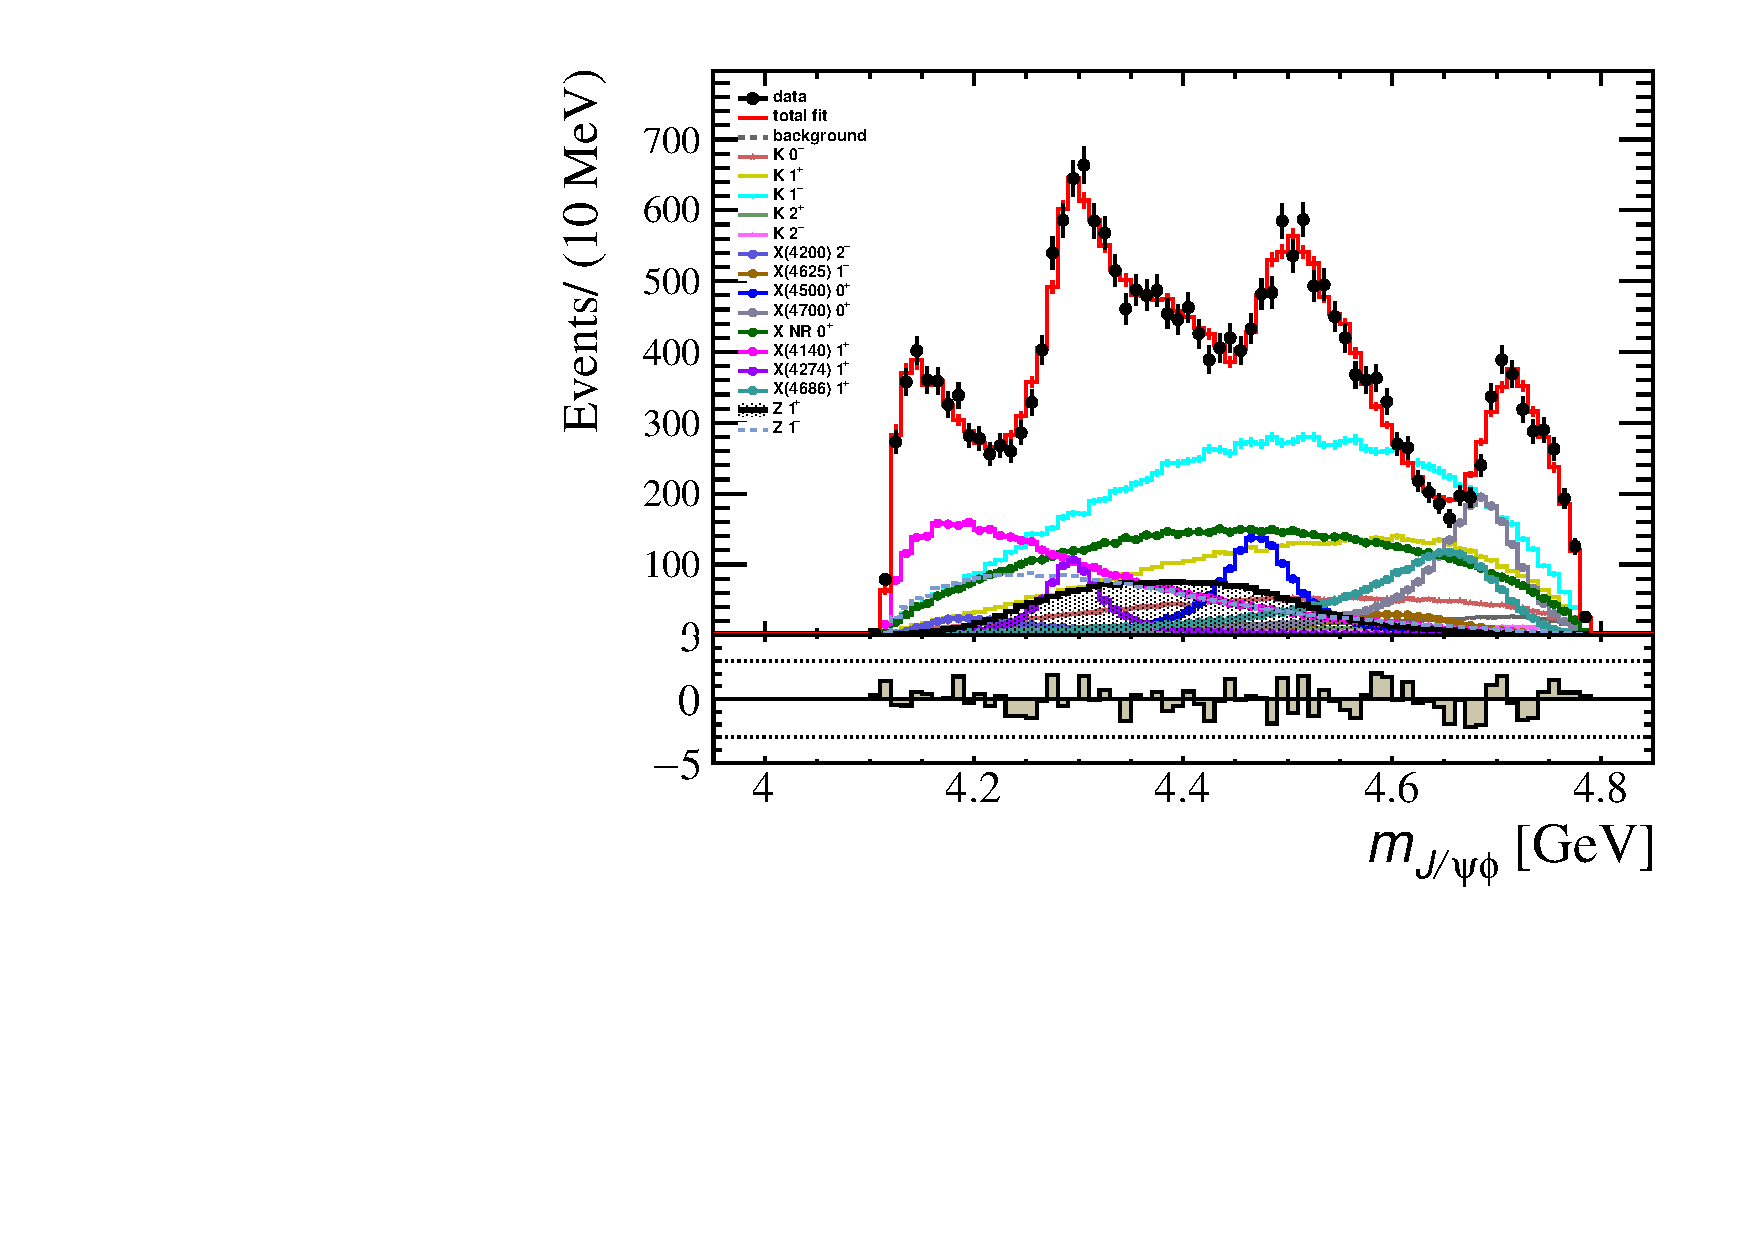
\includegraphics[width=0.5\textwidth]{Figures/06_Amplitude/Flatte/mjpsiphi-4140FL-Z1P}
\put(-50,140){\textrm{\small \bf(b)}}\\
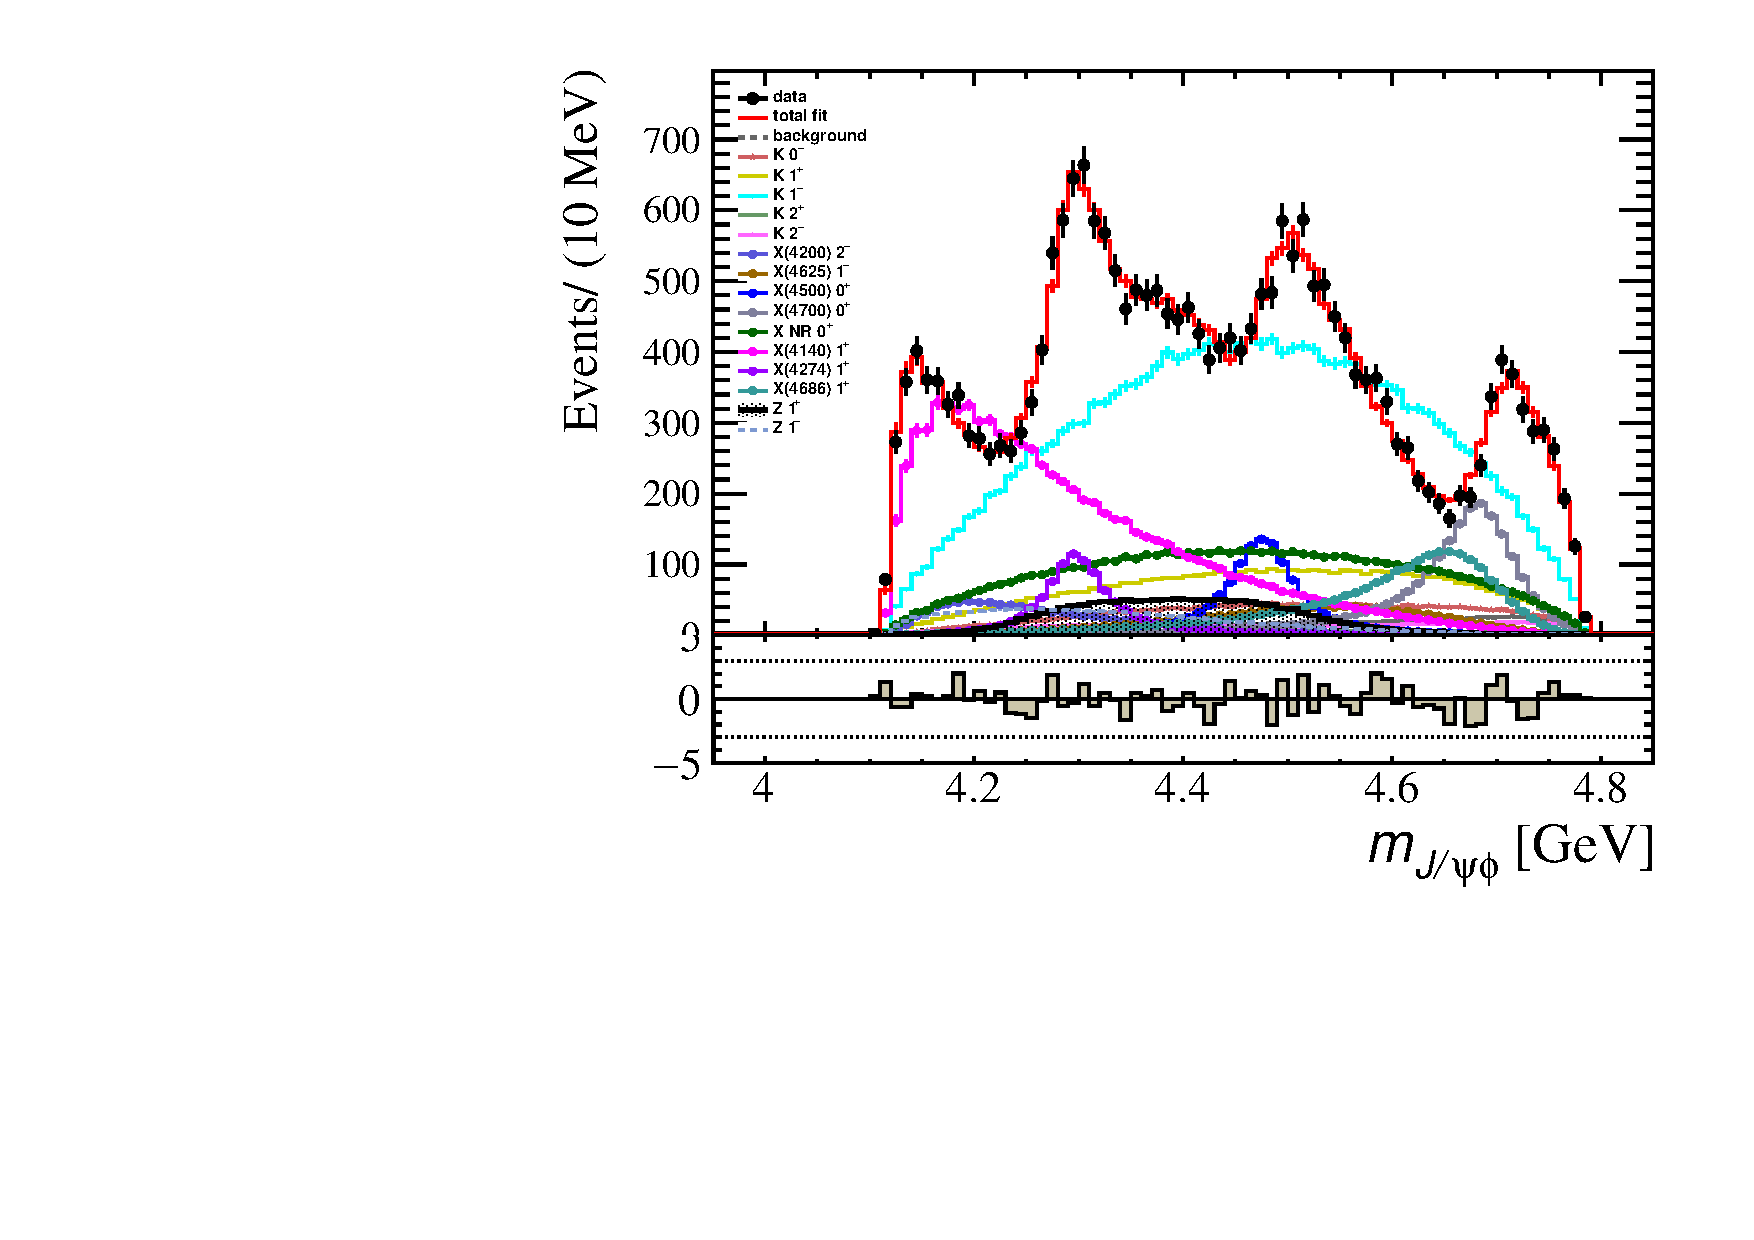
\includegraphics[width=0.5\textwidth]{Figures/06_Amplitude/Flatte/mjpsiphi-AllKFL-Z1M}%
\put(-50,140) {\textrm{\small \bf(c)}}%
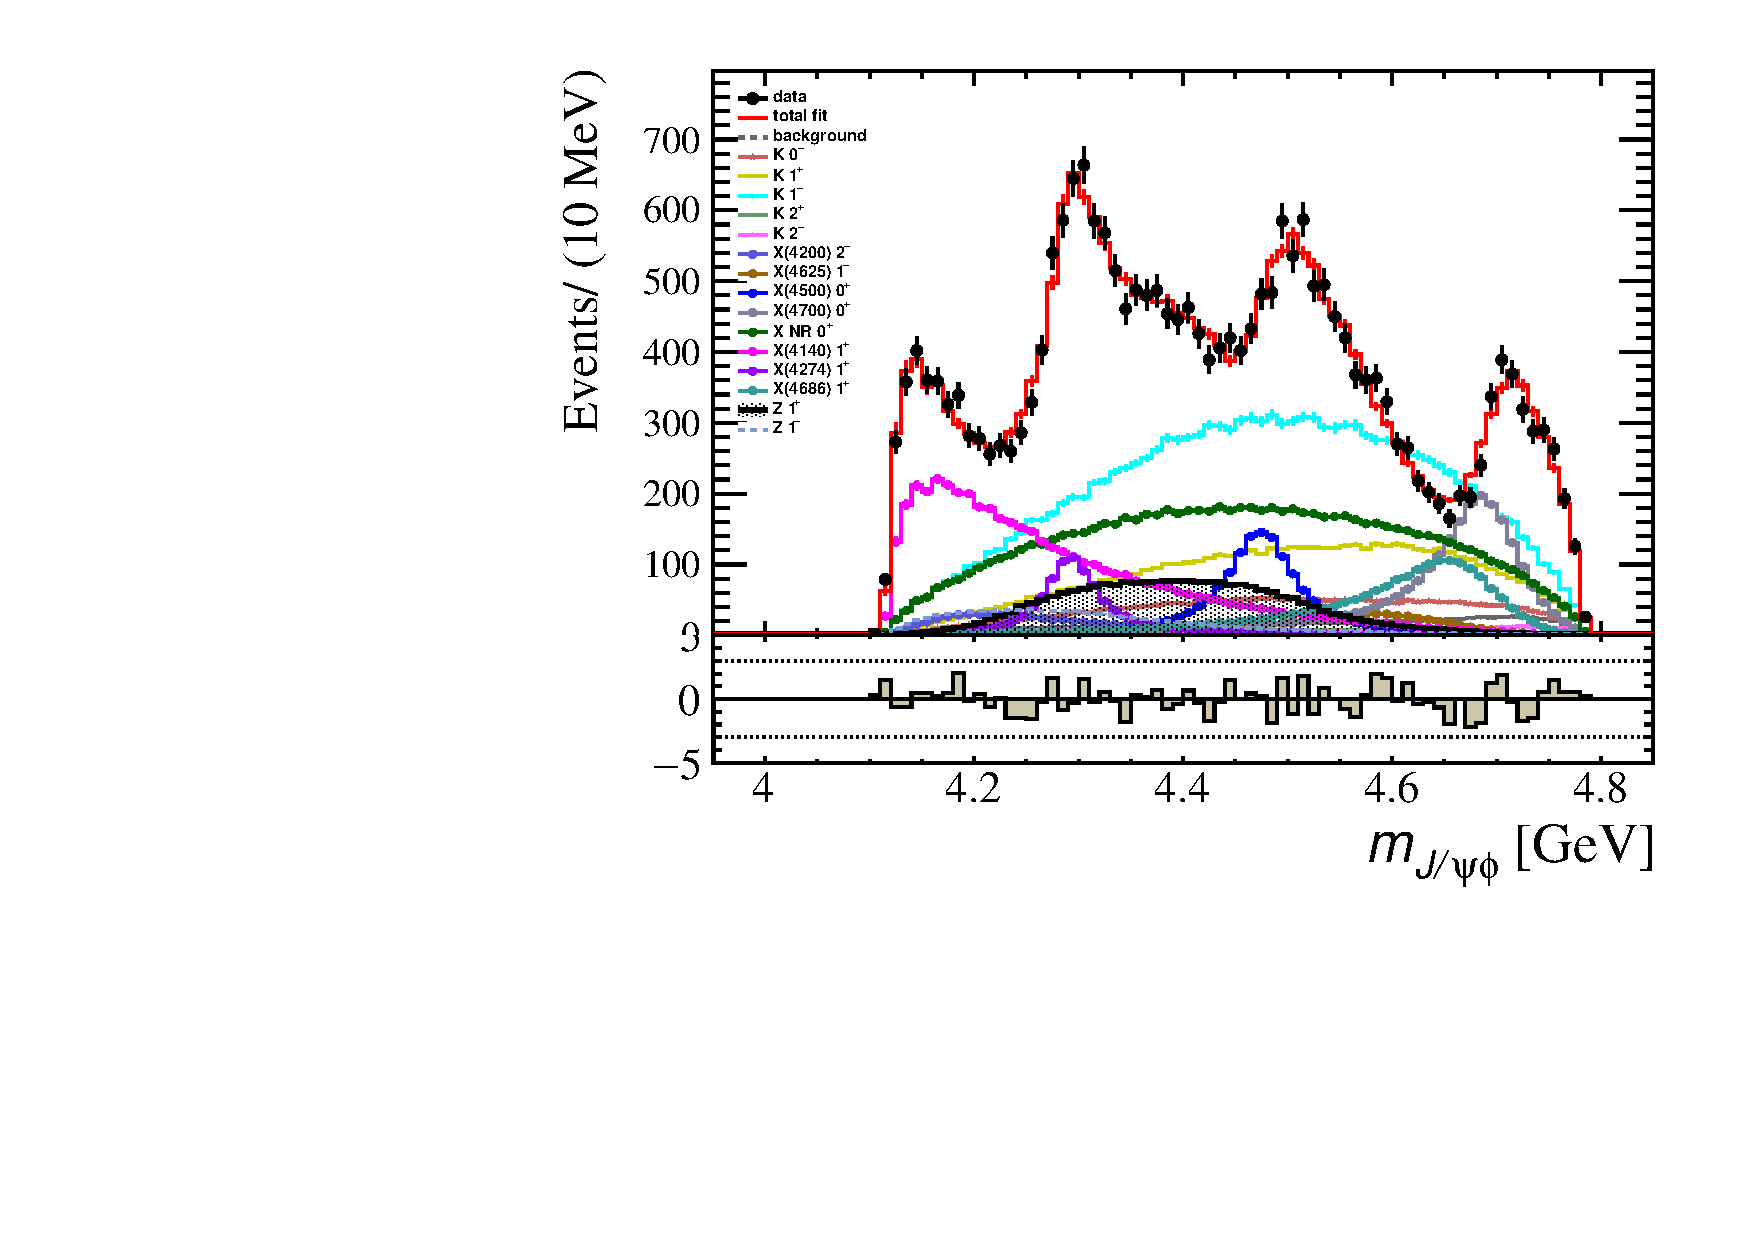
\includegraphics[width=0.5\textwidth]{Figures/06_Amplitude/Flatte/mjpsiphi-AllKFL-Z1P}
\put(-50,140){\textrm{\small \bf(d)}}
\caption{Projections of $\mjf$ from fits of Flatt\'e function for describing $\Xone$ in different resonance models 
(a) nominal $K$ and $1^-$ $Z(4220)$, (b) nominal $K$ and $1^+$ $Z_{cs}(4220)$, (c) extended $K$ and $1^-$ $Z_{cs}(4220)$, (b) extended $K$ and $1^+$ $Z(4220)$.}
\label{fig:flatte}
\end{figure*}

\begin{figure}[bt]
\centering
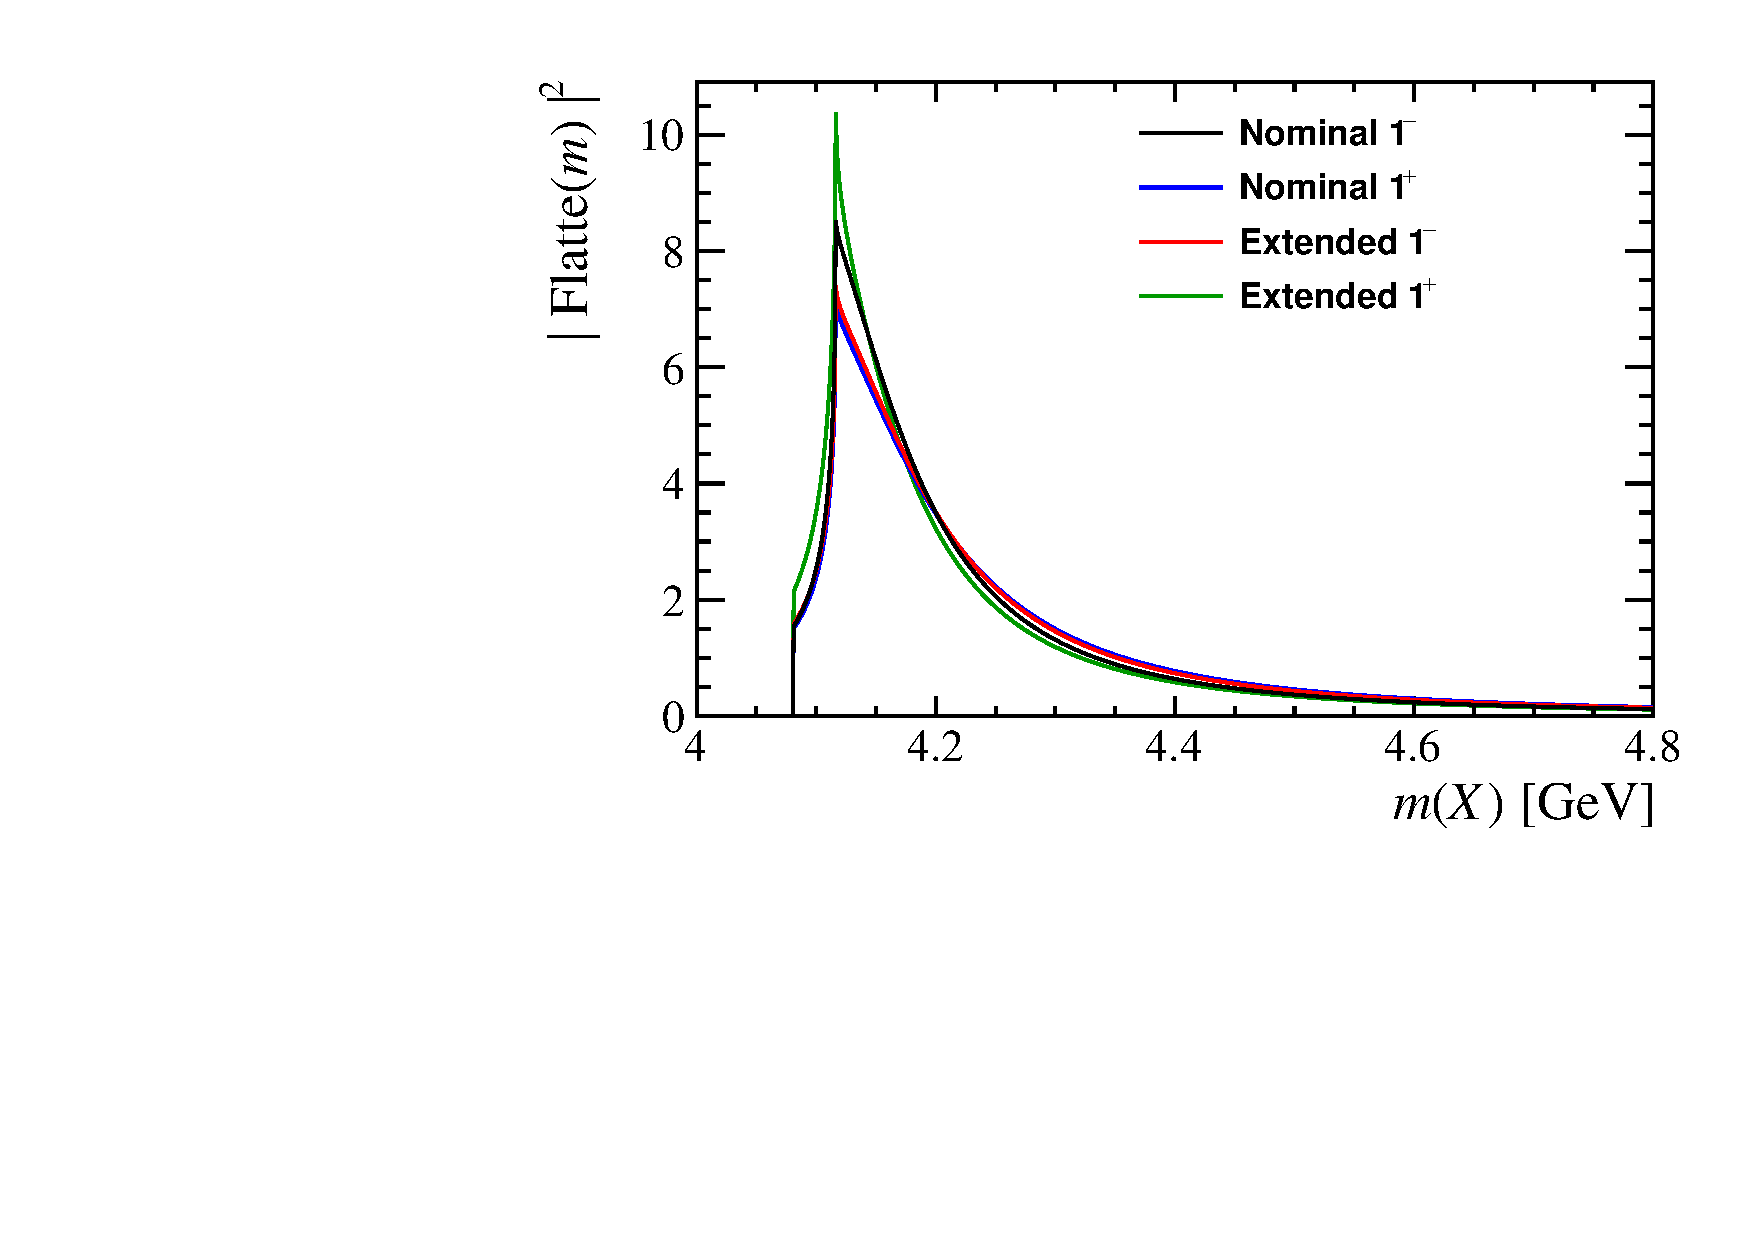
\includegraphics[width=0.65\textwidth]{Figures/06_Amplitude/Flatte/FlatteX}
\caption{Lineshapes of Flatt\'e parameterization of the $\Xone$ resonance.}\label{fig:cmpfl}
\end{figure}


The Flatt\'e $\Xone$ lineshapes, moduli of Eq.~(\ref{eq:fl}) squared, 
are compared in Fig.~\ref{fig:cmpfl}. 
Without the phase-space factor of $X\to\jpsi \phi$ decays, 
the lineshapes peak at the threshold. 
Similar results are obtained with the Breit-Wigner parameterization using constant width. 

Using Flatt\'e for $Z_{cs}(4000)^+$ is also investigated since it peaks close to the mass threshold of $\Dsp \Dstarzb$ and $\Dssp\Dzb$, 
assuming the same couplings for the two open charm channels. 
Also note that when $\mjk$ is below the mass threshold of one of the coupled channels, 
the channel's phase space factor becomes imagery. 
The fit is slightly better, $\Delta(-2\ln\Like)=2.8$,
but the improvement is not significant given that there is one addition free parameter in this model.
The fit results are $M^F_0=4029\pm22\mev$, $g_{\jpsi\Kp}=0.38\pm0.07\gev$, $(g_{\Dsp \Dstarzb}+g_{\Dssp\Dzb})/g_{\jpsi\Kp}=0.8\pm0.6$. 
While the coupling to $\jpsi\phi$ is significant, 
the coupling to the coupled-channels is not. 
However, within the large errors it is possible that the threshold plays an important role.
A pole for $Z_{cs}(4000)^+$ in Flatt\'e representation is found to be $M_0-i\Gamma_0/2=(4004\pm12 -i 91\pm22)$\mev. 
The statistical uncertainties are calculated by toy study where the correlations of the three parameters in Flatt\'e function are taken into account. 
The projection of this fit onto $\mjk$ is shown in Fig.~\ref{fig:FlatteZcs}.

\begin{figure*}[t]
\centering
%\begin{minipage}[b]{0.5\textwidth}
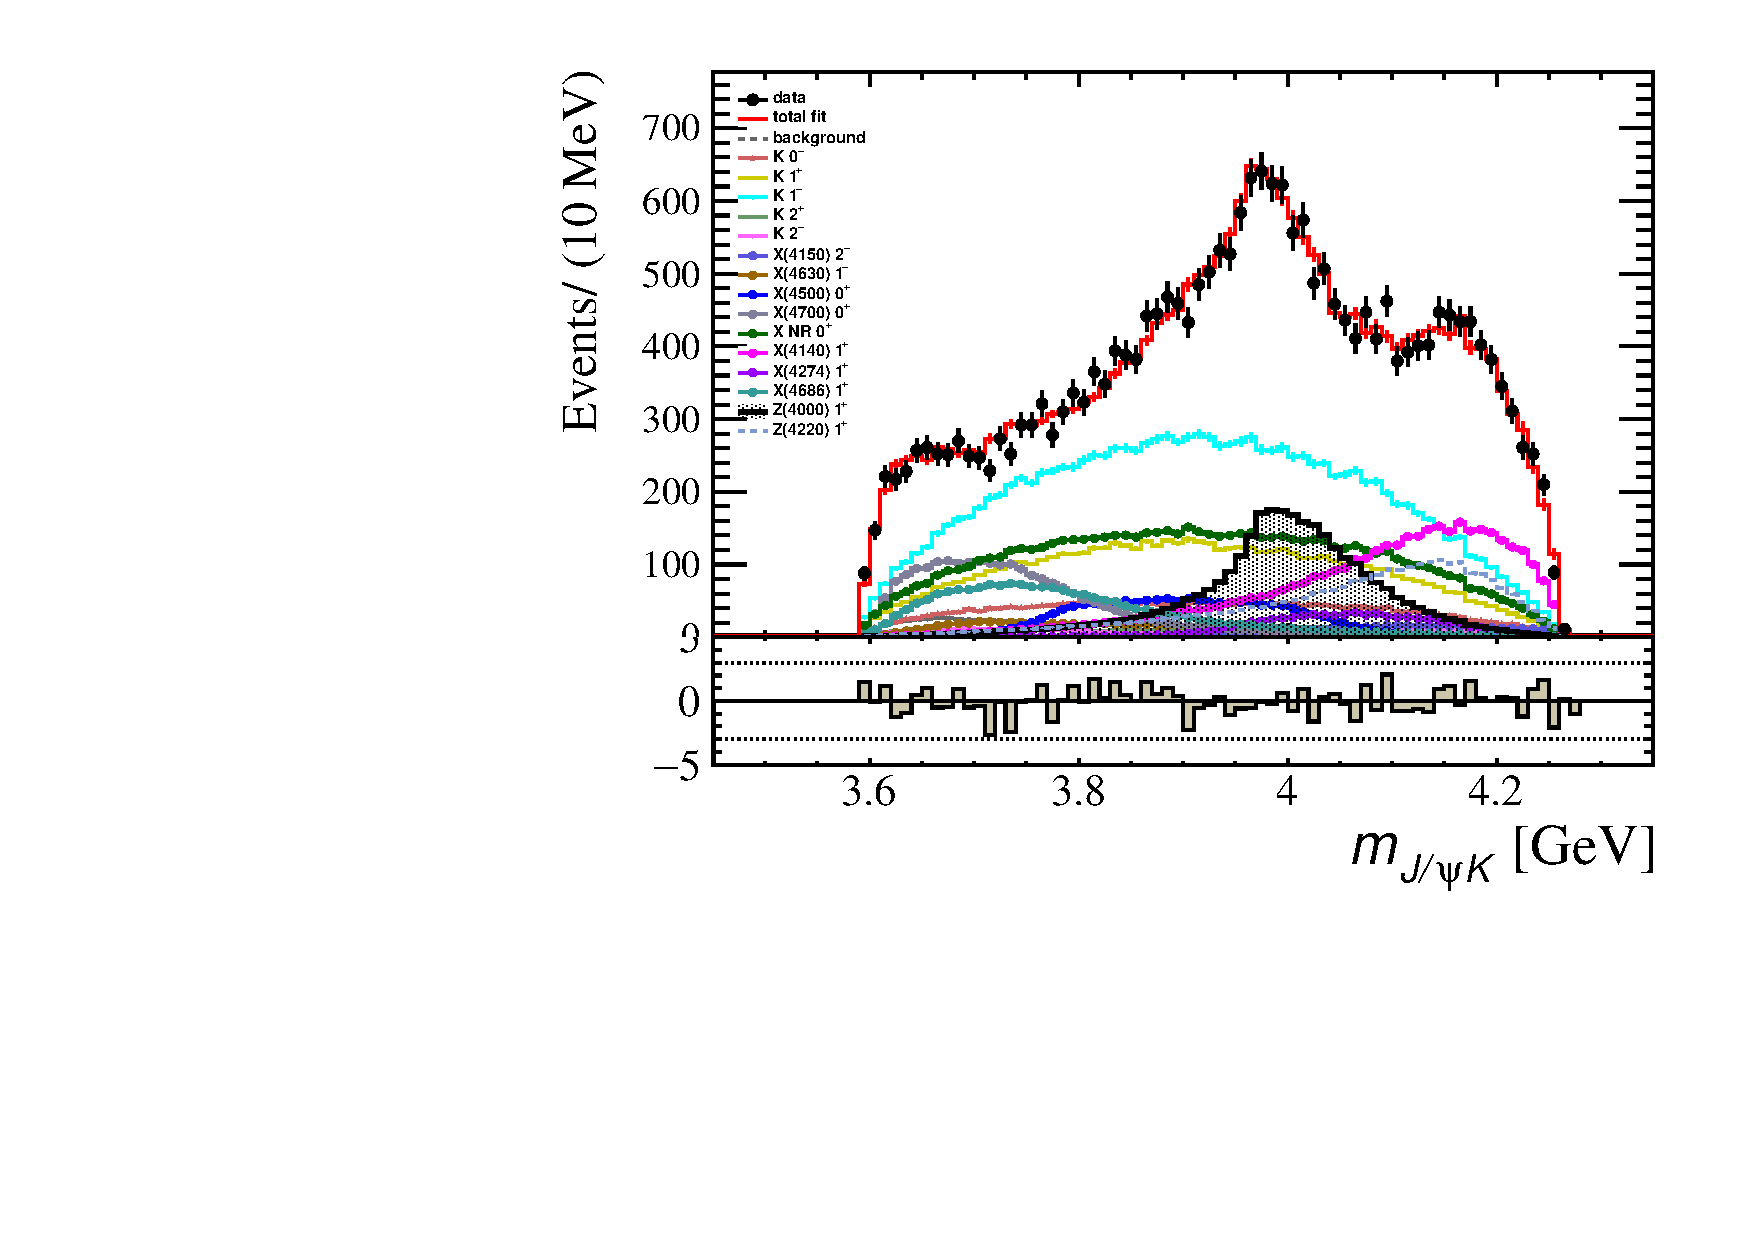
\includegraphics[width=0.6\textwidth]{Figures/06_Amplitude/Flatte/mjpsik-Z1PZFL}%
\caption{Projections onto $\mjk$ from the fit with the Flatt\'e function for describing $Z_{cs}(4000)^+$.}
\label{fig:FlatteZcs}
\end{figure*}

